\documentclass[11pt,a4paper]{report}
\usepackage[T1]{fontenc}
\usepackage[utf8]{inputenc}
\usepackage[portuguese]{babel}
\usepackage[margin=2cm]{geometry}
\usepackage{graphicx}
\usepackage{amsmath}
\usepackage{csquotes}
\usepackage{enumitem}
\usepackage{listings}
\usepackage{listing}
\usepackage[svgnames]{xcolor}
\usepackage{eurosym}
\usepackage{csvsimple}
\usepackage{biblatex}
\usepackage[bookmarks=true,unicode,pdfpagelabels]{hyperref}
\usepackage{bookmark}

\author{Carlos Pinto Machado
	<\href{mailto:2200909@estudante.uab.pt}{2200909@estudante.uab.pt}>}

\title{Exercícios Resolvidos da AULA AbERTA: Introdução à Estatística}

\addbibresource{bibliografia.bib}

\lstset{
	language=R,
	basicstyle=\footnotesize,
	numbers=left,
	numberstyle=\tiny\color{gray},
	stepnumber=1,
	numbersep=5pt,
	backgroundcolor=\color{white},
	showspaces=false,
	showstringspaces=false,
	showtabs=false,
	frame=single,
	rulecolor=\color{black},
	tabsize=4,
	captionpos=b,
	breaklines=true,
	breakatwhitespace=false,
	keywordstyle=\color{blue},
	commentstyle=\color{DarkGreen},
	escapeinside={\%*}{*)},
	literate=
		{á}{{\'a}}1 {é}{{\'e}}1 {í}{{\'i}}1 {ó}{{\'o}}1 {ú}{{\'u}}1
		{Á}{{\'A}}1 {É}{{\'E}}1 {Í}{{\'I}}1 {Ó}{{\'O}}1 {Ú}{{\'U}}1
		{à}{{\`a}}1 {è}{{\`e}}1 {ì}{{\`i}}1 {ò}{{\`o}}1 {ù}{{\`u}}1
		{À}{{\`A}}1 {È}{{\`E}}1 {Ì}{{\`I}}1 {Ò}{{\`O}}1 {Ù}{{\`U}}1
		{ä}{{\"a}}1 {ë}{{\"e}}1 {ï}{{\"i}}1 {ö}{{\"o}}1 {ü}{{\"u}}1
		{Ä}{{\"A}}1 {Ë}{{\"E}}1 {Ï}{{\"I}}1 {Ö}{{\"O}}1 {Ü}{{\"U}}1
		{â}{{\^a}}1 {ê}{{\^e}}1 {î}{{\^i}}1 {ô}{{\^o}}1 {û}{{\^u}}1
		{Â}{{\^A}}1 {Ê}{{\^E}}1 {Î}{{\^I}}1 {Ô}{{\^O}}1 {Û}{{\^U}}1
		{ã}{{\~a}}1 {ẽ}{{\~e}}1 {ĩ}{{\~i}}1 {õ}{{\~o}}1 {ũ}{{\~u}}1
		{Ã}{{\~A}}1 {Ẽ}{{\~E}}1 {Ĩ}{{\~I}}1 {Õ}{{\~O}}1 {Ũ}{{\~U}}1
		{œ}{{\oe}}1 {Œ}{{\OE}}1 {æ}{{\ae}}1 {Æ}{{\AE}}1 {ß}{{\ss}}1
		{ű}{{\H{u}}}1 {Ű}{{\H{U}}}1 {ő}{{\H{o}}}1 {Ő}{{\H{O}}}1
		{ç}{{\c c}}1 {Ç}{{\c C}}1 {ø}{{\o}}1 {Ø}{{\O}}1 {å}{{\r a}}1 {Å}{{\r A}}1
		{€}{{\euro}}1 {£}{{\pounds}}1 {«}{{\guillemotleft}}1
		{»}{{\guillemotright}}1 {ñ}{{\~n}}1 {Ñ}{{\~N}}1 {¿}{{?`}}1 {¡}{{!`}}1
		{º}{\textdegree}1
}

\begin{document}
\maketitle
\tableofcontents

\chapter{Introdução}

\paragraph{} No decorrer da AULA AbERTA - "Introdução à Estatística:
Estatística Descritiva com R"\cite{AulaAbertaIntroducaoEstatistica2017}, o
recurso formativo era um guia homónimo
\cite{OliveiraAulaAberta2017}, no qual existem
exercícios propostos. O presente documento pretende documentar soluções para o
mesmo com recurso à Bibliografia recomendada do mesmo
documento\cite{OliveiraEstatisticaDescritiva2011}.

\section{Notas de Implementação}

\paragraph{} Com recurso ao manual do R\cite{RManual}, existe uma tendência
aparente, que é a manipulação de data frames. Parece ser o nexo, sob qual o
ecosistema floresce. Por tal foi o foco nas soluções demonstradas, recorrendo
regularmente aos recursos disponíveis no site.

\paragraph{} Para carregamento dos dados e gestão dos dados, foram utilizados
ficheiros csv. Esta abordagem parece ser mais razoável, dado que
podemos ter ficheiros com milhares de amostras.


\section{Recursos associados}

\paragraph{} Na página do repositório\cite{a2edRRepo}
estão os recursos, código e datasets, em zip:

\begin{center}
	\url{https://github.com/cpmachado/a2edR/releases/latest}.
\end{center}


\setcounter{chapter}{2}
\chapter{Estatística Descritiva com R}
\section{Organização de dados no R}

\lstinputlisting[caption={ex3\_1.R}]{codigo/ex3_1.R}

\begin{table}[h!]
	\centering
	\csvreader[
		tabular = |c|c|r|l|,
		late after line = \\\hline,
		table head = \hline $i$ & $x_i$ & $n_i$ & $f_i$ \\ \hline
	]{tabela/ex3_1.csv}{xi=\xi, ni=\ni, fi=\sfi}{
		\thecsvrow & \xi & \ni & \sfi
	}
	\caption{Frequências simples e relativas de irmãos}
	\label{tab:3.1}
\end{table}

\clearpage

\section{Visualização de dados usando o R}

\begin{figure}[h!]
	\centering
	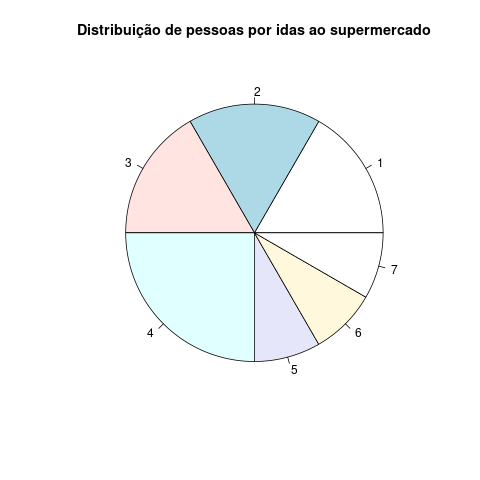
\includegraphics[width=0.7\textwidth]{imagem/ex3_2.png}
	\caption{Gráfico circular de idas ao supermercado}
\end{figure}
\lstinputlisting[caption={ex3\_2.R}]{codigo/ex3_2.R}

\clearpage
\section{Redução de dados: média aritmética e desvio padrão}

\begin{align*}
	\overline{x} &= 1.2\\
	s &\approx 1.067 \\
	\frac{s}{\overline{x}} &\approx 0.889 = 88.9 \%
\end{align*}

\paragraph{} A média permite-nos localizar a tendência central em redor dos
1.2 irmãos, e o desvio padrão de aproximadamente 1.067, permite-nos verificar
a dispersão associada. Sendo que o quociente do desvio padrão para com a média
é relativamente alto, permite-nos concluir que o esbatimento da curva é
rápido.

\paragraph{} Podemos verificar no gráfico \ref{fig:ex3_3} esse facto. Aparecem
também duas linhas a vermelho, demonstrando o conjunto de amostras no
intervalo com centro na média e raio de cumprimento do desvio
padrão($\overline{x} \pm s$). Data a natureza discreta da amostra fez-se uns
ajustes, sendo o intervalo dado por:

\begin{align*}
	\lceil \overline{x} - s \rceil &= \lceil 1.2 - 1.067 \rceil =  1 \\
	\lfloor \overline{x} + s \rfloor &= \lfloor 1.2 + 1.067 \rfloor = 2 \\
	I &= [\lceil \overline{x} - s \rceil, \lfloor \overline{x} + s \rfloor] =
	[1, 2]
\end{align*}


\begin{figure}[h!]
	\centering
	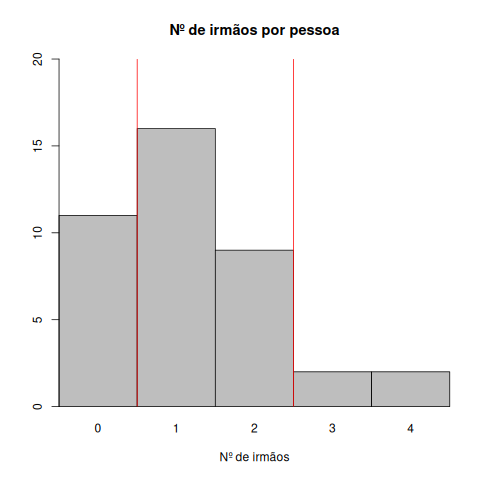
\includegraphics[width=0.7\textwidth]{imagem/ex3_3.png}
	\caption{Distribuição de irmãos por pessoa}
	\label{fig:ex3_3}
\end{figure}

\clearpage

\lstinputlisting[caption={ex3\_3.R}]{codigo/ex3_3.R}

\chapter{Exercícios}
\section*{Exercícios Propostos}

\begin{enumerate}[label=\arabic{chapter}.\arabic*]
	\item\addcontentsline{toc}{section}{4.1}\hfill
		\lstinputlisting[caption={ex4\_1.R}]{codigo/ex4_1.R}
		\begin{enumerate}[label=\alph*)]
		\item$\overline{x} = 19.41667$\hfill
		\item$s = 1.378954$\hfill
		\end{enumerate}
	\clearpage
	\item\addcontentsline{toc}{section}{4.2}\hfill
		\lstinputlisting[caption={ex4\_2.R}]{codigo/ex4_2.R}
		\begin{enumerate}[label=\alph*)]
		\item$N = 60$
		\item\hfill
			\begin{table}[h!]
				\centering
				\csvreader[
					tabular = |c|c|r|r|l|l|,
					late after line = \\\hline,
					table head = \hline $i$ & $x_i$ & $n_i$ & $N_i$
											& $f_i$ & $F_i$ \\ \hline
				]{tabela/ex4_2b.csv}
				{xi=\xi, ni=\ni, Ni=\Ni, fi=\sfi, Fi=\Fi}{
					\thecsvrow & \xi & \ni & \Ni & \sfi & \Fi
				}
				\caption{Tabela de frequências da distribuição de salários}
			\end{table}
		\item\hfill
			\begin{align*}
				\overline{x} &= 1260 \\
				s &= 54.5552122756449
			\end{align*}
	\clearpage
		\item\hfill
			\begin{figure}[h!]
				\centering
				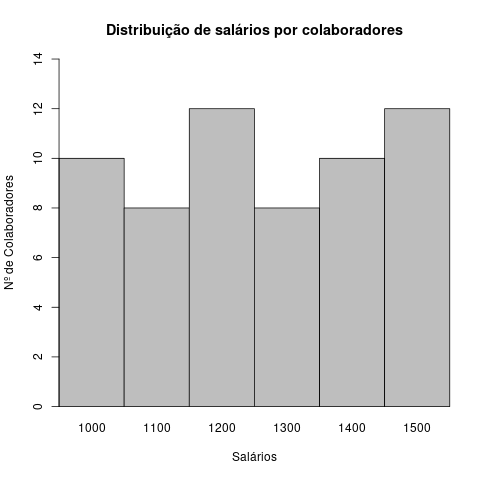
\includegraphics[width=0.6\textwidth]{imagem/ex4_2d.png}
				\caption{Distribuição dos salários por nº de colaboradores}
			\end{figure}
		\end{enumerate}
	\clearpage
	\item\addcontentsline{toc}{section}{4.3}\hfill
		\lstinputlisting[caption={ex4\_3.R}]{codigo/ex4_3.R}
		\begin{enumerate}[label=\alph*)]
		\item$\overline{x} = 64.26667$
		\item$s = 9.676678$
		\end{enumerate}
	\clearpage
	\item\addcontentsline{toc}{section}{4.4}\hfill
		\lstinputlisting[caption={ex4\_4.R}]{codigo/ex4_4.R}
		\begin{enumerate}[label=\alph*)]
		\item\hfill
			\begin{figure}[h!]
				\centering
				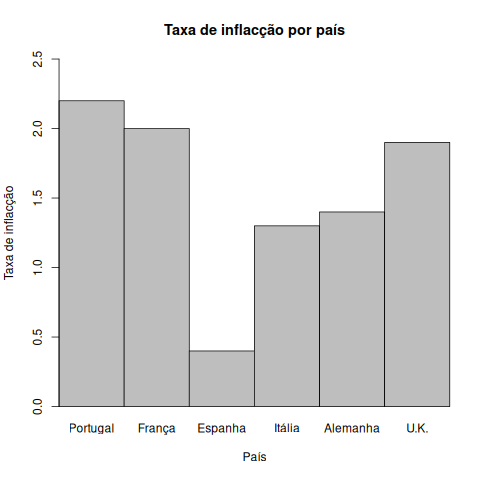
\includegraphics[width=0.5\textwidth]{imagem/ex4_4a.png}
				\caption{Taxa de Inflação por país}
			\end{figure}
	\clearpage
		\item\hfill
			\begin{figure}[h!]
				\centering
				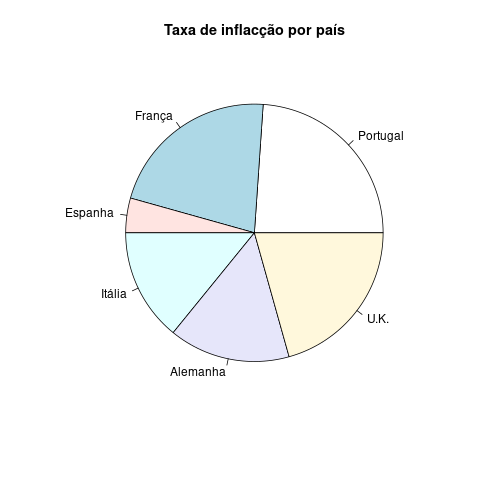
\includegraphics[width=0.5\textwidth]{imagem/ex4_4b.png}
				\caption{Taxa de inflação por país(Gráfico
				circular)}
			\end{figure}
		\item$\overline{x} = 1.533333$
		\end{enumerate}
\end{enumerate}

\bookmarksetup{startatroot}

\printbibliography[heading=bibintoc,title={Bibliografia}]
\begingroup
\let\clearpage\relax
\listoftables\addcontentsline{toc}{chapter}{Lista de Tabelas}
\listoffigures\addcontentsline{toc}{chapter}{Lista de Figuras}
\endgroup

\end{document}
